\section{Konwergencja i stabilność optymalizacji}
\label{sec:convergence-stability}

W tej sekcji przeanalizowano charakter optymalizacji dla sześciu reprezentantów fazy II, a celem jest ocena przebiegu procesu uczenia.

\begin{figure}[!ht]
\centering
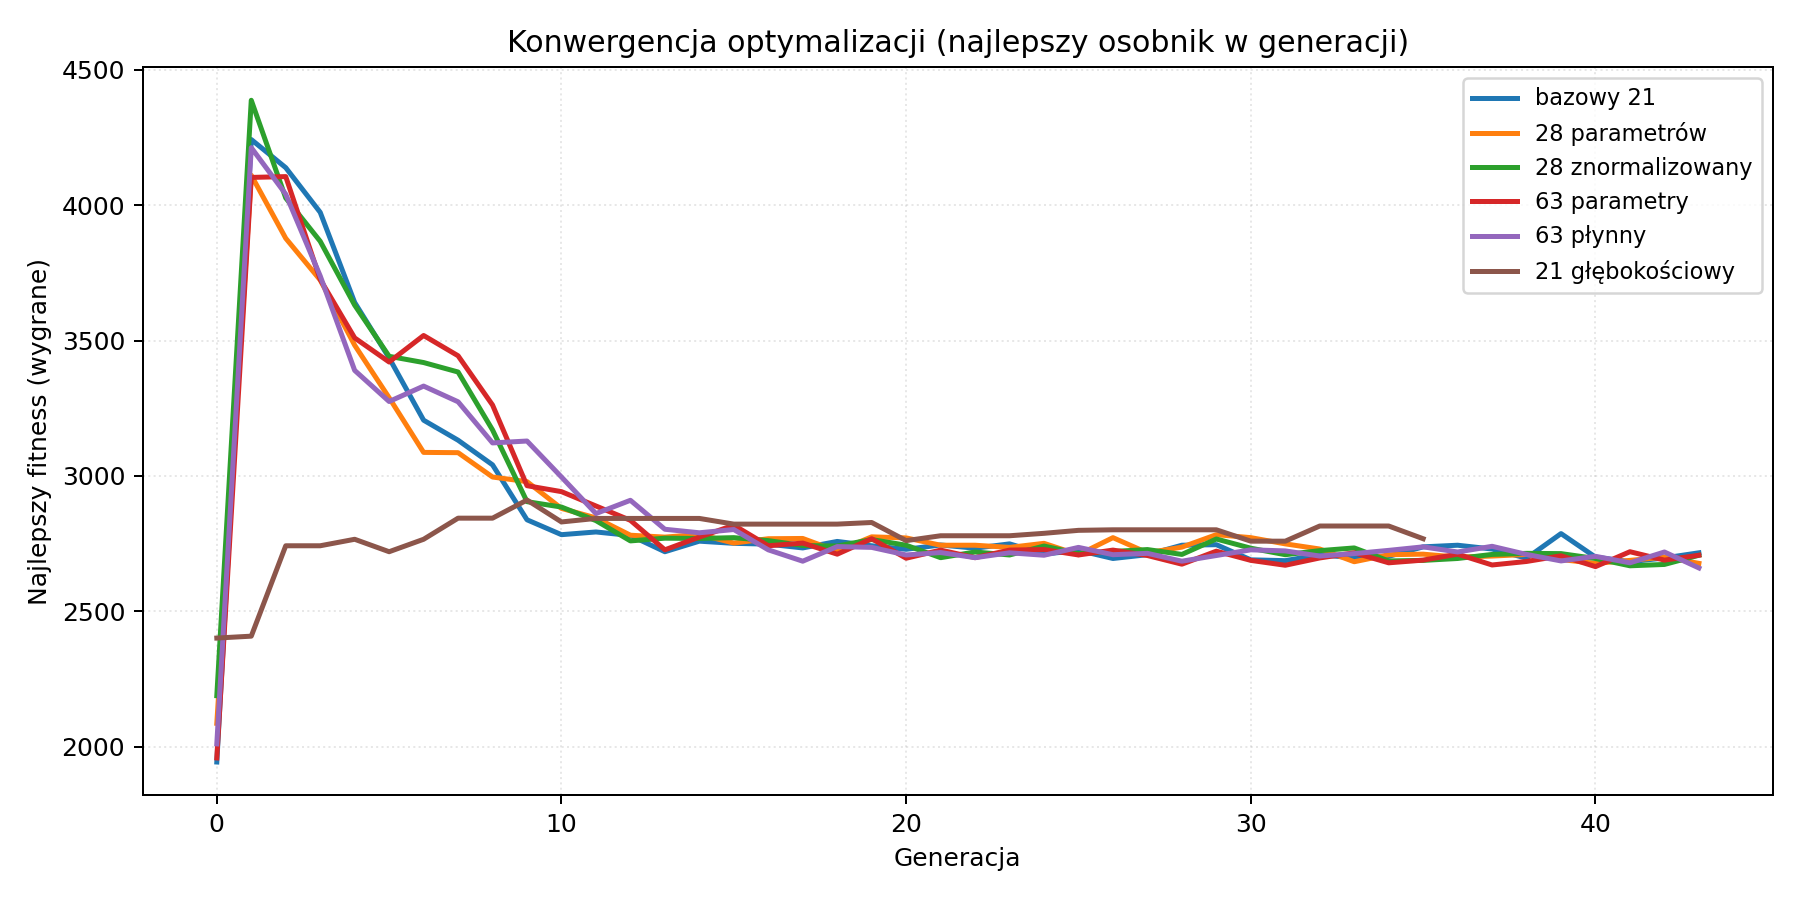
\includegraphics[width=0.95\textwidth]{chapters/07analysis/generated/figures/convergence_best_all.png}
\caption{Przebieg najlepszego osobnika w kolejnych generacjach dla sześciu reprezentantów fazy II.}
\label{fig:conv-best-all}
\end{figure}

\begin{figure}[!ht]
\centering
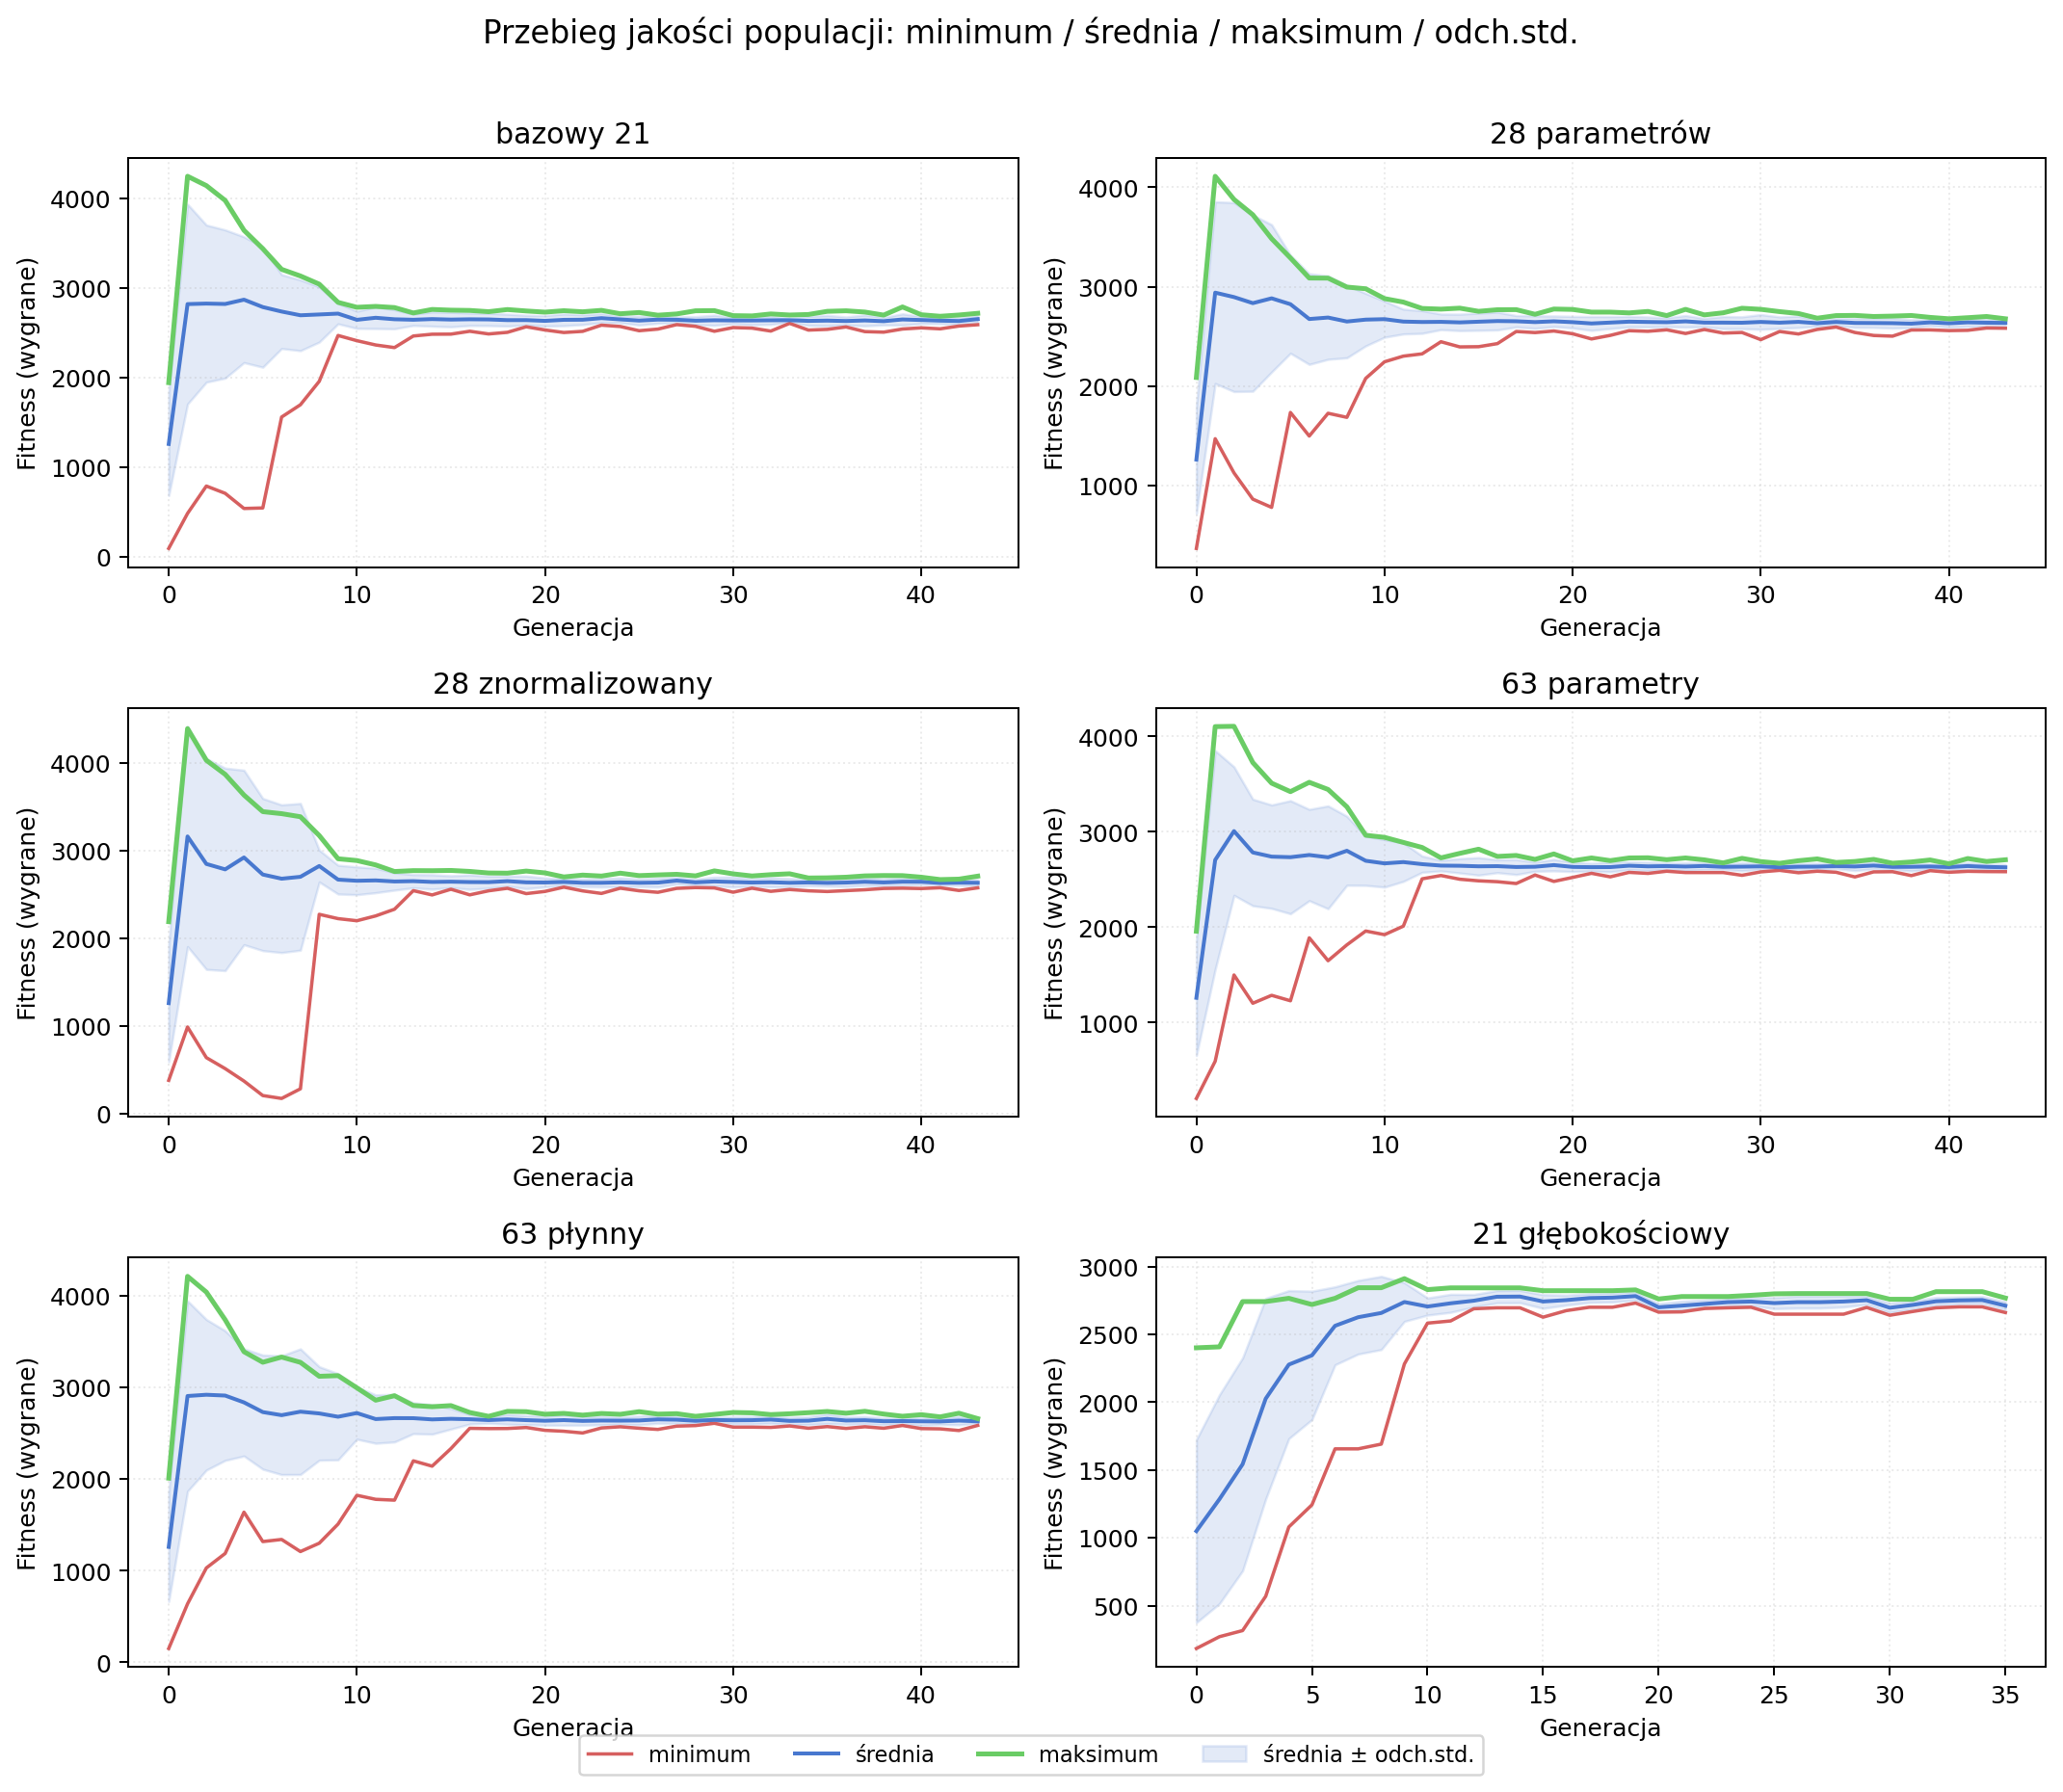
\includegraphics[width=0.98\textwidth]{chapters/07analysis/generated/figures/run_profiles_worst_mean_best_std.png}
\caption{Przebiegi jakości populacji: wartości minimalne, średnie i maksymalne oraz rozrzut jakości w kolejnych generacjach.}
\label{fig:run-profiles}
\end{figure}

Rysunek~\ref{fig:conv-best-all} należy czytać przede wszystkim jakościowo --- bezpośrednie porównanie wysokości krzywych między wariantami byłoby mylące. Pięciu reprezentantów wytrenowano za pomocą SHADE ze schematem koewolucyjnym, gdzie przystosowanie to suma wygranych w starciach z pozostałymi osobnikami bieżącej puli (równanie~\eqref{eq:fitness_coev}). Reprezentant wariantu \textit{21 głębokościowego} trenowany był natomiast SHADE z Hall of Fame --- przystosowanie liczone jest względem zbioru referencyjnego \(\mathcal{R}\) (równanie~\eqref{eq:fitness_hof}), aktualizowanego co \(5\) generacji. W obu przypadkach skala przystosowania ma charakter relatywny: gdy przeciwnicy stają się coraz lepsi, ten sam osobnik może uzyskać niższy wynik, mimo że w ujęciu absolutnym gra lepiej. Poziom osi \(y\) nie przekłada się więc wprost na ranking końcowy z fazy II.

Dla pięciu reprezentantów ze schematem koewolucyjnym widać podobny schemat --- mocny skok na początku, a potem spadek i wejście w stabilizację. Wczesny szczyt wynika z dużej różnicy siły między osobnikami w populacji startowej --- gdy reszta populacji się dostosowuje, nawet lepszy osobnik wygrywa mniej meczów względem silniejszych rywali. Naturalnym efektem jest dążenie wyników par do okolic \(50\%\), czyli stabilizacja sumy wygranych, niekoniecznie brak dalszej poprawy strategii. Wariant \textit{21 głębokościowy} ma spokojniejszy profil bez wysokiego szczytu startowego, co wynika z odmiennej logiki Hall of Fame. Zbiór referencyjny \(\mathcal{R}\) zawiera w większości silne, wytrenowane jednostki. Z tego powodu agenci muszą najpierw osiągnąć pewien poziom gry, zanim staną się wobec nich konkurencyjni --- stąd wolniejszy, ale bardziej równomierny wzrost przystosowania na początku procesu.

Rysunek~\ref{fig:run-profiles} pokazuje ten sam mechanizm na poziomie całej populacji. W pierwszych generacjach rosną jednocześnie minimum, średnia i maksimum. Po około 15. generacji większość przebiegów się wypłaszcza --- sygnał przystosowania przestaje wyraźnie rosnąć. Nie oznacza to jednak, że późniejsze generacje są nieistotne --- osobniki mogą nadal się doskonalić, ale wzrost siły przeciwników podczas ewaluacji maskuje ten postęp na wykresie. Końcową skuteczność agentów należy oceniać poprzez turniej, a nie przez absolutny poziom przystosowania z przebiegu optymalizacji.

To prowadzi do pytania, czy zwiększenie liczności populacji SHADE (\(\texttt{POP\_SIZE}=15\)) zmienia dynamikę tego sygnału i przekłada się na lepsze wyniki turniejowe --- mierzone na wspólnej, zewnętrznej skali gier.
\subsection{Analiza wrażliwości strojenia SHADE na liczność populacji}

\begin{figure}[!ht]
\centering
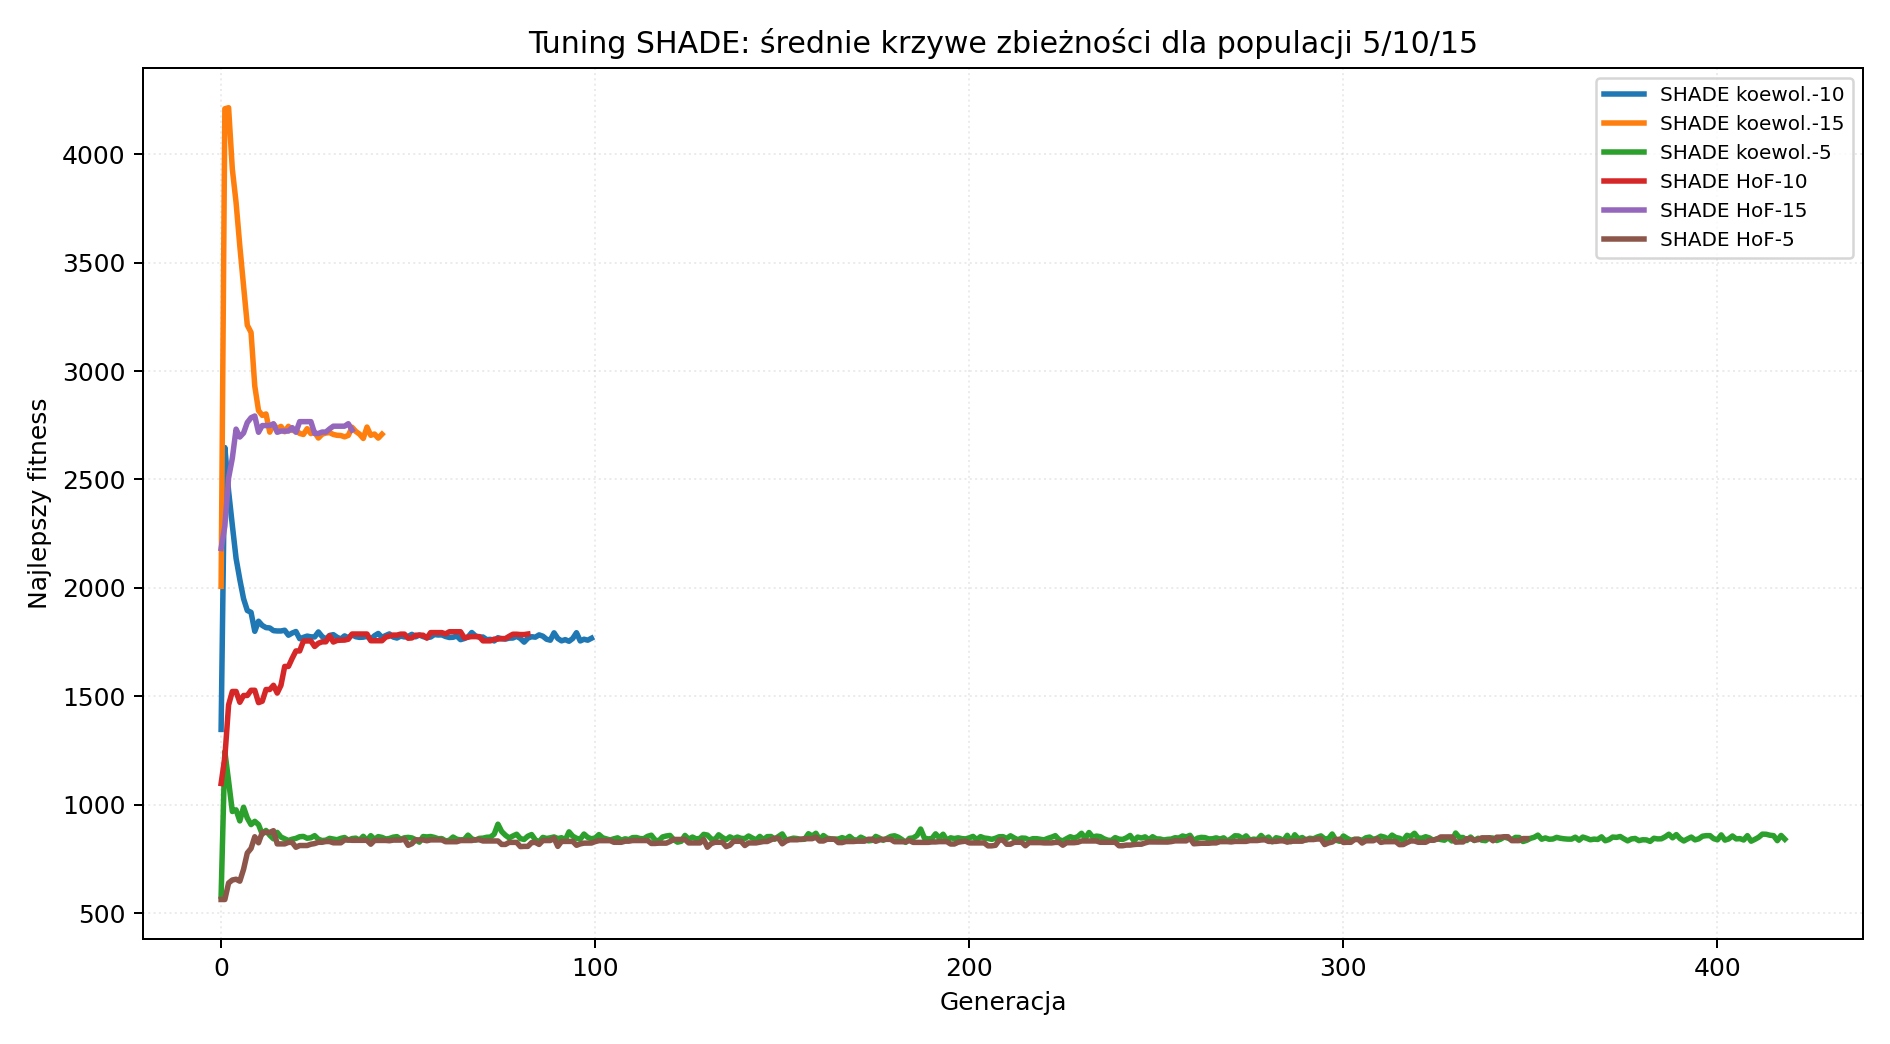
\includegraphics[width=0.96\textwidth]{chapters/07analysis/generated/figures/shade_tuning_convergence.png}
\caption{Dostrajanie parametrów SHADE: średnie krzywe zbieżności dla populacji 5, 10 i 15 (uśrednienie po dwóch zestawach wag dla każdej konfiguracji).}
\label{fig:shade-tuning-conv}
\end{figure}

\begin{figure}[!ht]
\centering
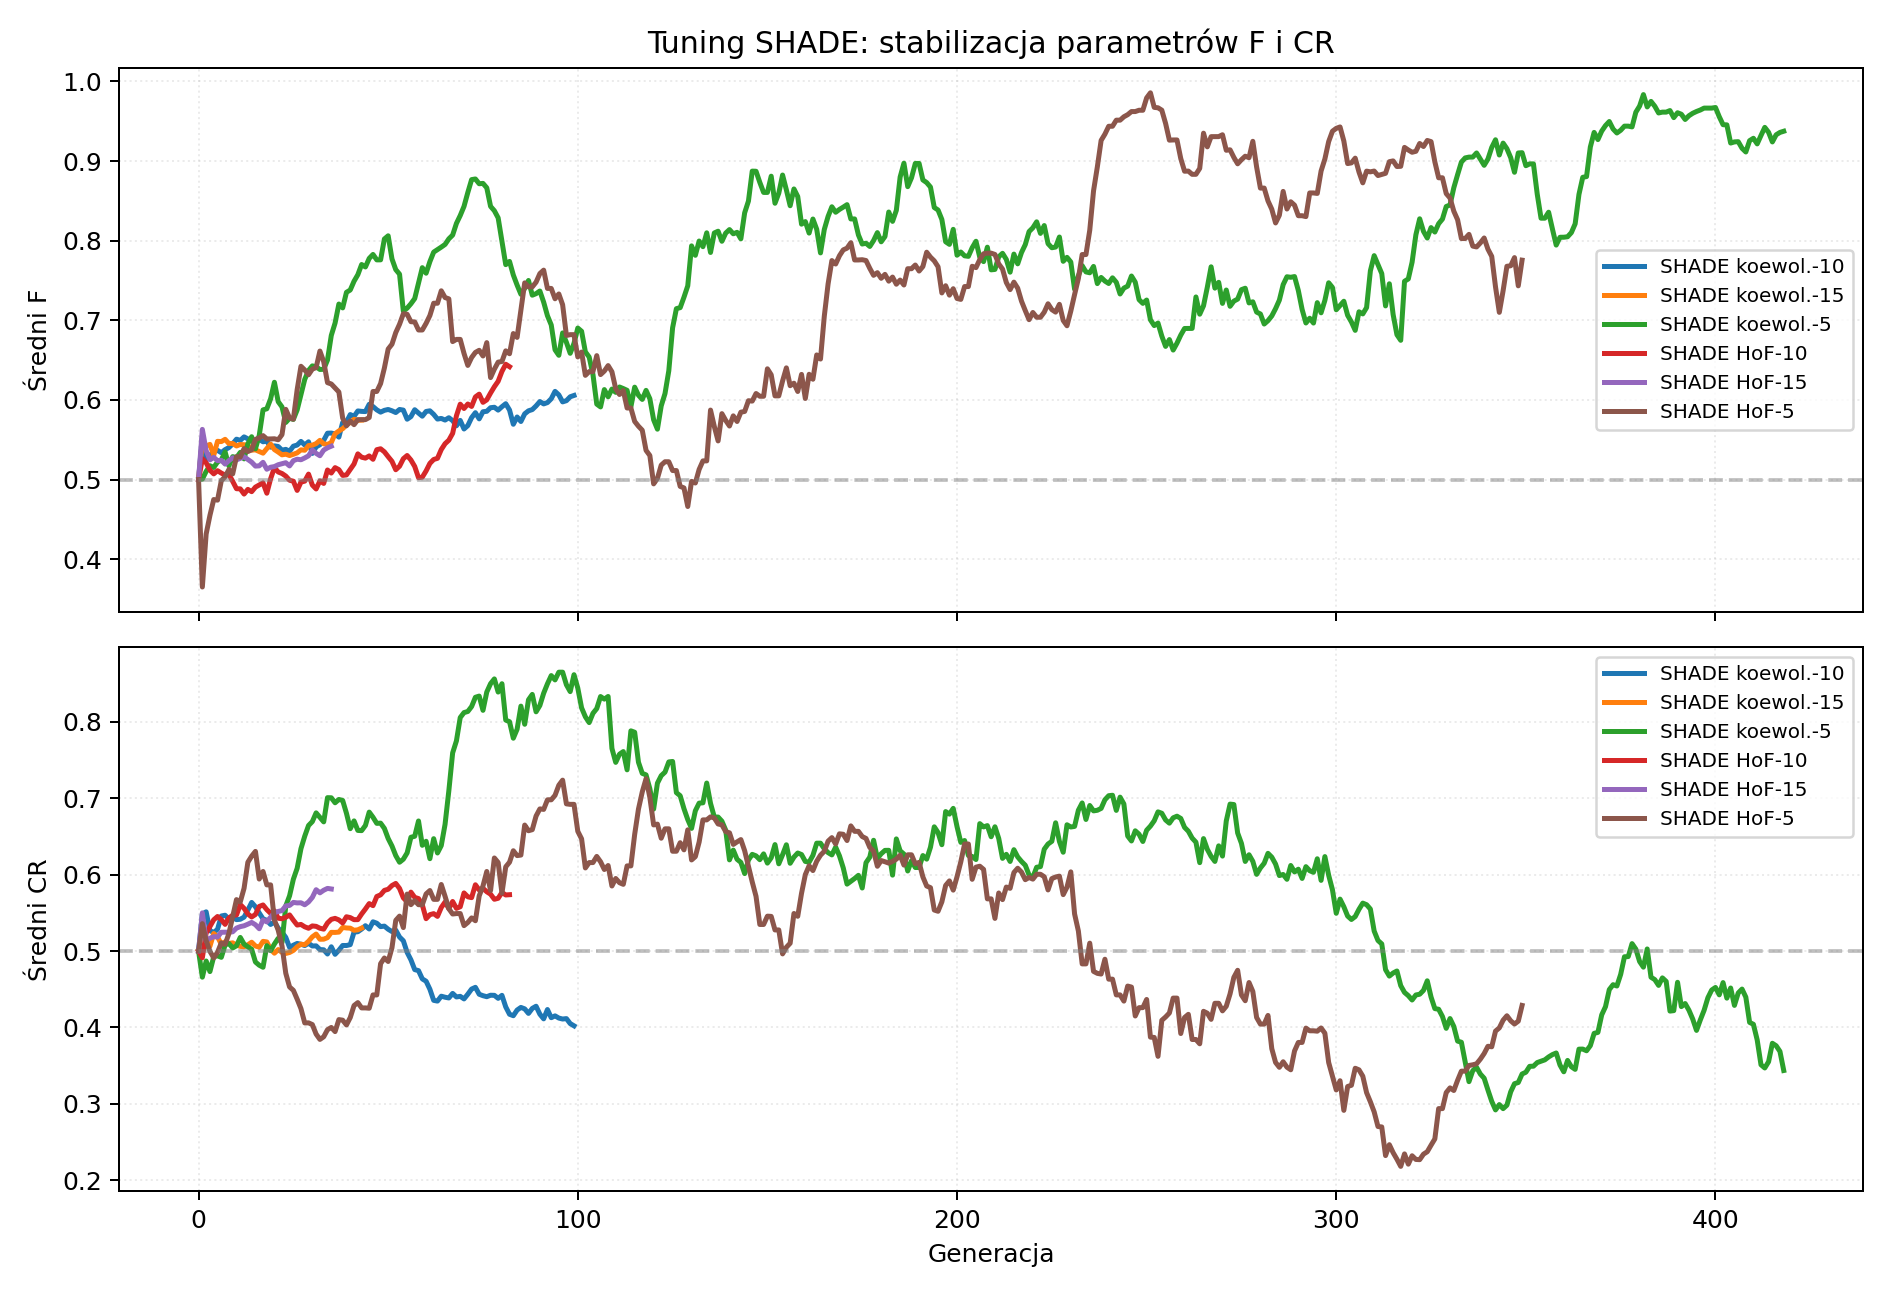
\includegraphics[width=0.96\textwidth]{chapters/07analysis/generated/figures/shade_tuning_f_cr.png}
\caption{Tuning SHADE: średnie przebiegi parametrów adaptacyjnych \(F\) i \(CR\) dla populacji 5, 10 i 15 (uśrednienie po dwóch zestawach wag dla każdej konfiguracji).}
\label{fig:shade-tuning-fcr}
\end{figure}

Wykresy z rysunków~\ref{fig:shade-tuning-conv} i~\ref{fig:shade-tuning-fcr} zbudowano jako średnią z dwóch zestawów wag dla każdej konfiguracji \((\texttt{POP\_SIZE},\) wariant SHADE\()\). Krzywe pokazują wspólny trend dla danej konfiguracji, natomiast tabela~\ref{tab:shade-popsize-results} prezentuje wyniki obu zestawów osobno.

Rysunek~\ref{fig:shade-tuning-conv} pokazuje szybkie wypłaszczenie krzywych przystosowania na trzech różnych poziomach. To naturalny efekt różnych skal ewaluacji dla \(\texttt{POP\_SIZE}=5/10/15\) --- każda konfiguracja miała inną liczbę przeciwników, więc wysokości krzywych nie należy porównywać wprost między sobą. W każdej konfiguracji największy przyrost pojawia się na początku, a późniejsze zmiany są małe. Wolniejszą stabilizację widać głównie dla wariantu z Hall of Fame z wielkością populacji 10.

Rysunek~\ref{fig:shade-tuning-fcr} pokazuje, że dla dłuższych przebiegów (zwłaszcza \(\texttt{POP\_SIZE}=5\)) średni \(F\) rośnie do wysokich wartości, podczas gdy \(CR\) z czasem często spada poniżej \(0{,}5\). Taki układ oznacza większe kroki mutacji przy bardziej zachowawczym krzyżowaniu --- algorytm mocniej przesuwa kandydatów, ale miesza mniej składowych naraz. Można to interpretować następująco, że przy małej populacji trudniej o stabilną poprawę drobnymi korektami --- częściej potrzebne są większe skoki, żeby wyrwać się z lokalnej stabilizacji. W tym sensie wyniki wspierają tezę, że w badanym budżecie obliczeniowym korzystniejsze jest szersze przeszukiwanie przestrzeni (większa populacja) niż dłuższe udoskonalanie małej. Dla populacji 10 i 15 przebiegi \(F\) i \(CR\) są krótsze i bliższe wartości startowej \(0{,}5\), ponieważ przy stałym budżecie ewaluacji wykonuje się mniej generacji.

Wyniki turnieju porównującego konfiguracje \(\texttt{POP\_SIZE}\in\{5,10,15\}\) dla obu wariantów SHADE zestawiono w tabeli~\ref{tab:shade-popsize-results}. W odróżnieniu od surowego przystosowania z przebiegu optymalizacji, wartości turniejowe wyrażone są jako wskaźnik wygranych w identycznym zestawie partii, co pozwala bezpośrednio porównywać skuteczność konfiguracji.

\begin{table}[!ht]
\centering
\small
\begin{tabular}{llrr}
\toprule
Wariant SHADE & Konfiguracja & \makecell{Wskaźnik wygranych\\(zestaw wag 1)} & \makecell{Wdsetek wygranych\\(zestaw wag 2)} \\
\midrule
\multirow{3}{*}{SHADE koewolucyjny}
    & POP\_SIZE = 5  & 48,64\% & 48,12\% \\
    & POP\_SIZE = 10 & 50,92\% & 48,51\% \\
    & POP\_SIZE = 15 & 52,15\% & 51,65\% \\
\midrule
\multirow{3}{*}{SHADE z Hall of Fame}
    & POP\_SIZE = 5  & 50,17\% & 44,77\% \\
    & POP\_SIZE = 10 & 51,37\% & 50,20\% \\
    & POP\_SIZE = 15 & 51,20\% & 52,30\% \\
\bottomrule
\end{tabular}
\caption{Wyniki turnieju doboru liczności populacji dla dwóch wariantów SHADE.}
\label{tab:shade-popsize-results}
\end{table}

Rysunki~\ref{fig:shade-tuning-conv} i~\ref{fig:shade-tuning-fcr} oraz tabela~\ref{tab:shade-popsize-results} dają spójny obraz --- większa populacja przeszukuje przestrzeń \emph{szerzej} kosztem mniejszej liczby kroków \emph{w głąb} przy stałym budżecie. Populacja 15 utrzymuje większą różnorodność kandydatów i osiąga nieco lepsze wyniki turniejowe. Mniejsze populacje szybciej zawężają przeszukiwanie, co widać także w szybszym wypłaszczeniu krzywych przystosowania.

Krzywe przystosowania reprezentantów fazy II szybko wypłaszczają się, odzwierciedla to stabilizację relatywnego sygnału selekcji przy użytych schematach ewaluacji, a nie bezpośrednio końcową siłę agentów. Większa populacja (\(15\)) daje nieco lepsze wyniki turniejowe niż \(5\) i \(10\) (tabela~\ref{tab:shade-popsize-results}), a turniej pozostaje właściwą miarą jakości.


















